\subsection{Coordinates of Point Dividing a Line in Ratio $k:1$}
\begin{definition}
({\em Budhayana's Theorem: })In Fig. \ref{fig:ch1_budhayana}, $ABC$ is a right angled triangle with $AB = b$ and $BC = c$.  Using coordinates, $A,B$ and $C$  can be represented as $\brak{a,b}, \brak{0,0}$ and $\brak{c,0}$, where $B$ is the origin, $BC$ is on the $X$-axis and $AB$ is on the $Y$-axis. Using Budhayana's theorem, $AC = \sqrt{b^2+c^2}$.
\end{definition}
%
\begin{figure}[!h]
\centering
\resizebox {\columnwidth} {!} {
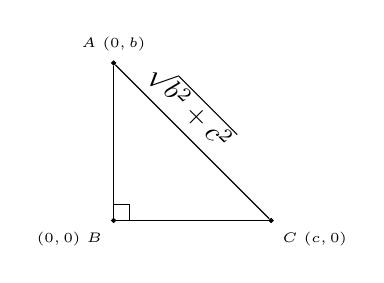
\begin{tikzpicture}
  [
    scale=2,
    >=stealth,
    point/.style = {draw, circle,  fill = black, inner sep = 0.5pt},
    dot/.style   = {draw, circle,  fill = black, inner sep = .2pt},
    every label/.append style={text=black, font=\tiny}
  ]
  \coordinate [point, label={below left:$(0,0)$ $B$}] (B) at (0, 0);
  \coordinate [point, label={above:$A$ $(0,b)$}] (A) at (0, 1);  
  \coordinate [point, label={below right:$C$ $(c,0)$}] (C) at (1,0);

  \path
     (A)    edge      (B)  
	 (B)    edge      (C)
	 (C)    edge  node[sloped, anchor=center, above, text width=2.0cm] { $\sqrt{b^2+c^2}$}     (A)	 
	 ;
  \newcommand{\ranglesize}{0.1cm}
  \draw (B) -- (0, \ranglesize) -- (\ranglesize, \ranglesize) --(\ranglesize, 0);


%  \draw  [line width=0.00mm ] (A) -- (C) -- (B) -- (A);

\end{tikzpicture}


}
\caption{Budhayana's Theorem}
\label{fig:ch1_budhayana}
\end{figure}
%%
\begin{problem}
Let $A$ and $B$ have the coordinates $\brak{a_1,a_2}$ and $\brak{b_1,b_2}$ respectively.  Show that the distance between $A$ and $B$ is given by 
%
\begin{equation}
\label{eq:ch1_distance}
AB = \sqrt{\brak{a_1 - b_1}^2 + \brak{a_2 - b_2}^2}
\end{equation}
%
\end{problem}
%
\renewcommand{\thefigure}{\theproblem.\arabic{figure}}
\begin{figure}[!h]
\centering
\resizebox {\columnwidth} {!} {
\begin{tikzpicture}
  [
    scale=2,
    >=stealth,
    point/.style = {draw, circle,  fill = black, inner sep = 0.5pt},
    dot/.style   = {draw, circle,  fill = black, inner sep = .2pt},
    every label/.append style={text=black, font=\tiny}
  ]
  \def\aa{2}
  \def\ab{3}    
  \def\ba{1}
  \def\bb{2}    
  \newcommand{\ranglesize}{0.1cm}  
  
  \coordinate [point, label={above right:$(a_1,a_2)$ $A$}] (A) at (\aa, \ab);
  \coordinate [point, label={below left:$(b_1,b_2)$ $B$}] (B) at (\ba, \bb);
  \coordinate [point, label={below left:$(0,0)$ $O$}] (O) at (0, 0);  
  \coordinate [point, label={below :$(a_1,0)$ $A_1$}] (A1) at (\aa, 0);  
  \coordinate [point, label={left:$(0,a_2)$ $A_2$}] (A2) at (0, \ab);  
  \coordinate [point, label={below :$(b_1,0)$ $B_1$}] (B1) at (\ba, 0);  
  \coordinate [point, label={left:$(0,b_2)$ $B_2$}] (B2) at (0, \bb);        
  \coordinate [point, label={right:$(a_1,b_2)$ $P$}] (P) at (\aa, \bb);    
  \path
     (A)    edge      (B)
     (O)    edge      (A1)     
     (O)    edge      (A2)          
     ;  
  \draw (O) -- (0, \ranglesize) -- (\ranglesize, \ranglesize) --(\ranglesize, 0);     
  \draw [dashed] 
  (A)  -- (A1)
  (A)  -- (A2)
  (P)  -- (B2)
  (B)  -- (B1);  

  
%  \coordinate [point, label={above:$A$ $(0,b)$}] (A) at (0, 1);  
%  \coordinate [point, label={below right:$C$ $(c,0)$}] (C) at (1,0);
%
%  \path
%     (A)    edge      (B)  
%	 (B)    edge      (C)
%	 (C)    edge  node[sloped, anchor=center, above, text width=2.0cm] { $\sqrt{b^2+c^2}$}     (A)	 
%	 ;

%  \draw (B) -- (0, \ranglesize) -- (\ranglesize, \ranglesize) --(\ranglesize, 0);


%  \draw  [line width=0.00mm ] (A) -- (C) -- (B) -- (A);

\end{tikzpicture}


}
\caption{Distance formula.}
\label{fig:ch1_distance}
\end{figure}
%
\renewcommand{\thefigure}{\theproblem.\arabic{figure}}
\begin{figure}[!h]
\centering
\resizebox {\columnwidth} {!} {
\begin{tikzpicture}
  [
    scale=2,
    >=stealth,
    point/.style = {draw, circle,  fill = black, inner sep = 0.5pt},
    dot/.style   = {draw, circle,  fill = black, inner sep = .2pt},
%    every label/.append style={text=black, font=\scriptsize}
  ]
  \def\aa{3}
  \def\ab{4}    
  \def\ba{2}
  \def\bb{3}    
  \newcommand{\ranglesize}{0.1cm}  
  
  \coordinate [point, label={above right:$(a_1,a_2)$ $A$}] (A) at (\aa, \ab);
  \coordinate [point, label={below left:$(b_1,b_2)$ $B$}] (B) at (\ba, \bb);
  \coordinate [point, label={below left:$(0,0)$ $O$}] (O) at (0, 0);  
  \coordinate [point, label={below :$(a_1,0)$ $A_1$}] (A1) at (\aa, 0);  
  \coordinate [point, label={left:$(0,a_2)$ $A_2$}] (A2) at (0, \ab);  
  \coordinate [point, label={below :$(b_1,0)$ $B_1$}] (B1) at (\ba, 0);  
  \coordinate [point, label={left:$(0,b_2)$ $B_2$}] (B2) at (0, \bb);        
  \coordinate [point, label={right:$(a_1,b_2)$ $P$}] (P) at (\aa, \bb); 
  \coordinate [point, label={below:$\substack{(a_1-b_1,0) \\ P^{'}}$}] (PP) at (\aa-\ba, 0);         
  \coordinate [point, label={right:$\substack{(a_1-b_1,a_2-b_2) \\ A^{\prime}}$ }] (AP) at (\aa-\ba, \ab-\bb);  
%  \coordinate [point, label={right:$(a_1,b_2)$ $P$}] (P) at (0, \ab-\bb);           
  \path
     (A)    edge      (B)
     (O)    edge      (A1)     
     (O)    edge      (A2)          
     ;  
  \draw (O) -- (0, \ranglesize) -- (\ranglesize, \ranglesize) --(\ranglesize, 0);     
  \draw [dashed] 
  (A)  -- (A1)
  (A)  -- (A2)
  (P)  -- (B2)
  (B)  -- (B1)
  (O)  -- (AP)
  (PP)  -- (AP)  
  ;  

  
%  \coordinate [point, label={above:$A$ $(0,b)$}] (A) at (0, 1);  
%  \coordinate [point, label={below right:$C$ $(c,0)$}] (C) at (1,0);
%
%  \path
%     (A)    edge      (B)  
%	 (B)    edge      (C)
%	 (C)    edge  node[sloped, anchor=center, above, text width=2.0cm] { $\sqrt{b^2+c^2}$}     (A)	 
%	 ;

%  \draw (B) -- (0, \ranglesize) -- (\ranglesize, \ranglesize) --(\ranglesize, 0);


%  \draw  [line width=0.00mm ] (A) -- (C) -- (B) -- (A);

\end{tikzpicture}


}
\caption{Alternative visualization of distance.}
\label{fig:ch1_distance_shift}
\end{figure}

\renewcommand{\thefigure}{\theproblem}
%
\proof In Fig. \ref{fig:ch1_distance}, it is obvious that 
\begin{align}
PB &=A_1B_1 = a_1-b_1
\\
PA &= A_2B_2 = a_2-b_2 
\end{align}
%
Using Budhayana's theorem, 
%
\begin{equation}
AB = \sqrt{PA^2+PB^2} = \sqrt{\brak{a_1 - b_1}^2 + \brak{a_2 - b_2}^2}
\end{equation}
%
An alternative visualization of Fig. \ref{fig:ch1_distance} is available in \ref{fig:ch1_distance_shift}, where the line $AB$ is shifted to the origin such that the line becomes $A^{\prime}O$.  This results in  
\begin{equation}
OA^{\prime} = \sqrt{\brak{A^{\prime}P^{\prime}}^2 + \brak{O^{\prime}P^{\prime}}^2} = \sqrt{\brak{a_1 - b_1}^2 + \brak{a_2 - b_2}^2}
\end{equation}
%
Thus, shifting the coordinates by $\brak{b_1,b_2}$ makes the visualization as well as computation easier.  This trick will be used quite a lot in this book.
\begin{problem}
In Fig. \ref{fig:ch1_ratio}, $P$ divides $AB$ in the ratio $k:1$ such that
\begin{equation}
\frac{PA}{PB} = k.
\end{equation}
If the coordinates of $A$ and $B$ are $\brak{a_1,a_2}$ and
$\brak{b_1,b_2} $ respectively, show that the coordinates of $P$ are
\begin{equation}
\label{eq:ch1_ratio}
\brak{\frac{a_1+kb_1}{k+1},\frac{a_2+kb_2}{k+1}}
\end{equation}
\end{problem}
%

\begin{figure}[!h]
\centering
\resizebox {\columnwidth} {!} {
\begin{tikzpicture}
  [
    scale=2,
    >=stealth,
    point/.style = {draw, circle,  fill = black, inner sep = 0.5pt},
    dot/.style   = {draw, circle,  fill = black, inner sep = .2pt},
%    every label/.append style={text=black, font=\tiny}
  ]
  \def\aa{3}
  \def\ab{3}    
  \def\ba{1}
  \def\bb{1}    
  \newcommand{\ranglesize}{0.1cm}  
  
  \coordinate [point, label={above right:$(a_1,a_2)$ $A$}] (A) at (\aa, \ab);
  \coordinate [point, label={below left:$(b_1,b_2)$ $B$}] (B) at (\ba, \bb);
  \coordinate [point, label={below left:$(0,0)$ $O$}] (O) at (0, 0);  
  \coordinate [point, label={below :$(a_1,0)$ $A_1$}] (A1) at (\aa, 0);  
  \coordinate [point, label={left:$(0,a_2)$ $A_2$}] (A2) at (0, \ab);  
  \coordinate [point, label={below :$(b_1,0)$ $B_1$}] (B1) at (\ba, 0);  
  \coordinate [point, label={left:$(0,b_2)$ $B_2$}] (B2) at (0, \bb);        
  \coordinate [point, label={right:$(a_1,b_2)$ }] (Pt) at (\aa, \bb);    
  \node (P) at ($(A)!0.5!(B)$) [point, label = {above left:$P$ $\brak{x,y}$}]{};  
  \node (P1) at ($(A1)!0.5!(B1)$) [point, label = {below:$P_1$ $\brak{x,0}$}]{};    
  \path
     (A)    edge  node[sloped, anchor=center, above, text width=2.0cm] { $k:1$}     (B)       
     (O)    edge      (A1)     
     (O)    edge      (A2)          
     ;  
  \draw (O) -- (0, \ranglesize) -- (\ranglesize, \ranglesize) --(\ranglesize, 0);     
  \draw [dashed] 
  (A)  -- (A1)
  (A)  -- (A2)
  (Pt)  -- (B2)
  (B)  -- (B1)
  (P)  -- (P1);  

  
%  \coordinate [point, label={above:$A$ $(0,b)$}] (A) at (0, 1);  
%  \coordinate [point, label={below right:$C$ $(c,0)$}] (C) at (1,0);
%
%  \path
%     (A)    edge      (B)  
%	 (B)    edge      (C)
%	 (C)    edge  node[sloped, anchor=center, above, text width=2.0cm] { $\sqrt{b^2+c^2}$}     (A)	 
%	 ;

%  \draw (B) -- (0, \ranglesize) -- (\ranglesize, \ranglesize) --(\ranglesize, 0);


%  \draw  [line width=0.00mm ] (A) -- (C) -- (B) -- (A);

\end{tikzpicture}


}
\caption{$P$ divides $AB$ in the ratio $k:1$.}
\label{fig:ch1_ratio}
\end{figure}
%
\proof From Fig. \ref{fig:ch1_ratio}, using similar triangles, it is obvious that
%
\begin{equation}
\frac{PB}{PA} = \frac{P_1B_1}{P_1A_1} = \frac{x-b_1}{a_1-x} = k
\end{equation}
%
Simplifying the above, 
%
\begin{align}
x - b_1 &= k\brak{a_1-x}
\\
\Rightarrow \brak{1+k}x & = ka_1+b_1
\\
\Rightarrow x &= \frac{ka_1+b_1}{k+1}
\end{align}
%
The proof for $y$ is similar.
%
\subsection{Median}
\begin{definition}
	The line segment $AD$ in Fig. \ref{fig:ch1_median_def} that divides the side $BC$ in two equal halfs ($BD=DC$) is known as the median.
\end{definition}
%
\begin{figure}[!h]
\centering
\resizebox {\columnwidth} {!} {
\begin{tikzpicture}
  [
    scale=2,
    >=stealth,
    point/.style = {draw, circle,  fill = black, inner sep = 0.5pt},
    dot/.style   = {draw, circle,  fill = black, inner sep = .2pt},
  ]
  \coordinate [point, label={below left:$B$}] (B) at (0, 0);
    \node (A) at +(60:{2*sqrt(3)}) [point, label = above:$A$] {};
  \coordinate [point, label={below right:$C$}] (C) at ($ (3,0) + sqrt(3)*(1,0) $);

  \draw  (A) -- (C) -- (B) -- (A);
  \node (D) at ($(B)!0.5!(C)$) [point, label = {below:$D$}]{};
  \draw (A) -- (D);  

\end{tikzpicture}


}
\caption{Median}
\label{fig:ch1_median_def}
\end{figure}
%

\begin{problem}
The medians $BE$ and $CF$ in Fig. \ref{fig:ch1_two_median} intersect at $O$, such that
\begin{equation}
\begin{split}
\frac{OB}{OE} &= k_1
\\
\frac{OC}{OF} &= k_2
\end{split}
\end{equation}
Show that $k_1 = k_2 = 2$.
\end{problem}
%
\begin{figure}[!h]
\centering
\resizebox {\columnwidth} {!} {
\begin{tikzpicture}
  [
    scale=2,
    >=stealth,
    point/.style = {draw, circle,  fill = black, inner sep = 0.5pt},
    dot/.style   = {draw, circle,  fill = black, inner sep = .2pt},
  ]
  \coordinate [point, label={below left:$B$ $(0, 0)$}] (B) at (0, 0);
    \node (A) at +(60:{2*sqrt(3)}) [point, label = above:$A$ ${(a,b)}$  ] {};
  \coordinate [point, label={below left:$(c,0)$ $C$ }] (C) at ($ (3,0) + sqrt(3)*(1,0) $);

  \draw  (A) -- (C) -- (B) -- (A);
  \node (E) at ($(A)!0.5!(C)$) [point, label = {right:$E$}]{};
  \node (F) at ($(A)!0.5!(B)$) [point, label = {left:$F$}]{};
  \path
     (B)    edge  node[sloped, anchor=center, below, text width=2.0cm] { $k_1:1$}     (E)  
	 (C)    edge  node[sloped, anchor=east, below, text width=2.0cm] { $1:k_2$}     (F);
  \node (O) at ($(B)!0.67!(E)$) [point, label = {below:$O$}]{};  
\end{tikzpicture}


}
\caption{Medians $BE$ and $CF$}
\label{fig:ch1_two_median}
\end{figure}
\proof
Let the coordinates of $A$, $B$ and $C$ be $\brak{a,b}$, $\brak{0,0}$ and $\brak{c,0}$ respectively. Using \ref{eq:ch1_ratio}, 
%
\begin{align}
E = 
\begin{pmatrix}
\frac{a+c}{2}
\\
\frac{b}{2}
\end{pmatrix}
\\
F = 
\begin{pmatrix}
\frac{a}{2}
\\
\frac{b}{2}
\end{pmatrix}
\end{align}
%
Since $O$ divides $BE$ in the ratio $k_1:1$, from \eqref{eq:ch1_ratio},
\begin{align}
O &= \frac{k_1E+B}{k_1+1}
= \frac{1}{k_1+1}\sbrak{k_1
\begin{pmatrix}
\frac{a+c}{2}
\\
\frac{b}{2}
\end{pmatrix}
+
\begin{pmatrix}
0
\\
0
\end{pmatrix}
}
\\
&= \frac{k_1}{2\brak{k_1+1}}
\begin{pmatrix}
a+c
\\
b
\end{pmatrix}
\label{eq:ch1_ratio_1}
\end{align}
%
Similarly, since $O$ divides $CF$ in the ratio $k_2:1$,
\begin{align}
O &= \frac{k_2F+C}{k_2+1} = \frac{1}{k_2+1}\sbrak{
k_2
\begin{pmatrix}
\frac{a}{2}
\\
\frac{b}{2}
\end{pmatrix}
+
\begin{pmatrix}
c
\\
0
\end{pmatrix}
}
\\
&= \frac{1}{2\brak{k_2+1}}
\begin{pmatrix}
ak_2+2c
\\
bk_2
\end{pmatrix}
\label{eq:ch1_ratio_2}
\end{align}
From \eqref{eq:ch1_ratio_1} and \eqref{eq:ch1_ratio_2},
\begin{align}
\frac{k_1}{2\brak{k_1+1}}
\begin{pmatrix}
a+c
\\
b
\end{pmatrix}
&=
\frac{1}{2\brak{k_2+1}}
\begin{pmatrix}
ak_2+2c
\\
bk_2
\end{pmatrix}
\\
\Rightarrow
\frac{k_1}{\brak{k_1+1}}
\begin{pmatrix}
a+c
\\
b
\end{pmatrix}
&=
\frac{1}{\brak{k_2+1}}
\begin{pmatrix}
ak_2+2c
\\
bk_2
\end{pmatrix}
\end{align}
By equating the respective coordinates,
%
\begin{align}
\label{eq:ch1_ratio_3}
\frac{k_1\brak{a+c}}{k_1+1} &= \frac{ak_2+2c}{k_2+1}
\\
\frac{k_1b}{k_1+1} &= \frac{k_2b}{k_2+1}
\label{eq:ch1_ratio_4}
\end{align}
%
From \eqref{eq:ch1_ratio_4}, it is trivial to obtain $k_1=k_2$.  Substituting this in \eqref{eq:ch1_ratio_3} and simplifying,
\begin{align}
k_1\brak{a+c} &= ak_1 + 2c
\\
\Rightarrow k_1 = 2
\end{align}
Thus $k_1=k_2=2$.
\begin{problem}
In Fig.\ref{fig:ch1_two_median_conv},
\begin{equation}
\frac{OB}{OE} = \frac{OC}{OF} = 2
\end{equation}
Show that $BE$ and $CF$ are medians.
\end{problem}
%
\begin{figure}[!h]
\centering
\resizebox {\columnwidth} {!} {
\begin{tikzpicture}
  [
    scale=2,
    >=stealth,
    point/.style = {draw, circle,  fill = black, inner sep = 0.5pt},
    dot/.style   = {draw, circle,  fill = black, inner sep = .2pt},
  ]
  \coordinate [point, label={below left:$B$ $(0, 0)$}] (B) at (0, 0);
    \node (A) at +(60:{2*sqrt(3)}) [point, label = above:$A$ ${(a,b)}$  ] {};
  \coordinate [point, label={below left:$(c,0)$ $C$ }] (C) at ($ (3,0) + sqrt(3)*(1,0) $);

%  \draw  (A) -- (C) -- (B) -- (A);
  \node (E) at ($(A)!0.5!(C)$) [point, label = {right:$E$}]{};
  \node (F) at ($(A)!0.5!(B)$) [point, label = {left:$F$}]{};
  \path
     (A)    edge  node[sloped, anchor=center, below, text width=2.0cm] { $1:k_1$}     (B)    
     (A)    edge  node[sloped, anchor=center, above, text width=2.0cm] { $k_2:1$}     (C)         
     (B)		edge  (C)
     (B)    edge  node[sloped, anchor=center, below, text width=2.0cm] { $2:1$}     (E)  
	 (C)    edge  node[sloped, anchor=east, below, text width=2.0cm] { $1:2$}     (F);
  \node (O) at ($(B)!0.67!(E)$) [point, label = {below:$O$}]{};  
\end{tikzpicture}


}
\caption{$O$ divides $BE$ and $CF$ in the ratio $2:1$.}
\label{fig:ch1_two_median_conv}
\end{figure}
\proof  Let $E$ divide $AC$ in the ratio $k_2:1$ and $F$ divide $AB$ in the ratio $k_1:1$. Using \eqref{eq:ch1_ratio},
\begin{align}
E &= \frac{k_2C+A}{k_2+1} = \frac{1}{k_2+1}\sbrak{k_2
\begin{pmatrix}
c
\\
0
\end{pmatrix}
+
\begin{pmatrix}
a
\\
b
\end{pmatrix}
}
\\
&=
\frac{1}{k_2+1}
\begin{pmatrix}
k_2c+a
\\
b
\end{pmatrix}
\end{align}
and
\begin{align}
F &= \frac{k_1B+A}{k1+1} = \frac{1}{k_1+1}\sbrak{k_1
\begin{pmatrix}
0
\\
0
\end{pmatrix}
+
\begin{pmatrix}
a
\\
b
\end{pmatrix}
}
\\
&=
\frac{1}{k_1+1}
\begin{pmatrix}
a
\\
b
\end{pmatrix}
\end{align}
Since $O$ divides $BE$ in the ratio $2:1$, using \eqref{eq:ch1_ratio},
\begin{align}
O &= \frac{2E+B}{3} = \frac{2}{3\brak{k_2+1}}
\begin{pmatrix}
k_2c+a
\\
b
\end{pmatrix}
\label{eq:ch1_Oratio_1}
\end{align}
Also, $O$ divides $CF$ in the ratio $2:1$, hence,
%
\begin{align}
O &= \frac{2F+C}{3} = \frac{1}{3}
\sbrak{\frac{2}{k_1+1}
\begin{pmatrix}
a
\\
b
\end{pmatrix}
+
\begin{pmatrix}
c
\\
0
\end{pmatrix}
}
\\
&=
\frac{1}{3\brak{k_1+1}}
\begin{pmatrix}
2a+\brak{k_1+1}c
\\
2b
\end{pmatrix}
\label{eq:ch1_Oratio_2}
\end{align}
%
Equating \eqref{eq:ch1_Oratio_1} and \eqref{eq:ch1_Oratio_2},
\begin{align}
\frac{2}{3\brak{k_2+1}}
\begin{pmatrix}
k_2c+a
\\
b
\end{pmatrix}
&=
\frac{1}{3\brak{k_1+1}}
\begin{pmatrix}
2a+\brak{k_1+1}c
\\
2b
\end{pmatrix}
\\
\Rightarrow
\frac{2}{\brak{k_2+1}}
\begin{pmatrix}
k_2c+a
\\
b
\end{pmatrix}
&=
\frac{1}{\brak{k_1+1}}
\begin{pmatrix}
2a+\brak{k_1+1}c
\\
2b
\end{pmatrix}
\end{align}
Equating the respective coordinates,
\begin{align}
\label{eq:ch1_Oratio_3}
\frac{2\brak{k_2c+a}}{3\brak{k_2+1}} &= \frac{2a+\brak{k_1+1}c}{k_1+1}
\\
\frac{2b}{k_2+1} &= \frac{2b}{k_1+1}
\label{eq:ch1_Oratio_4}
\end{align}
From \eqref{eq:ch1_Oratio_4}, $k_1=k_2$ is trivially obtained.  Substituting this in \eqref{eq:ch1_Oratio_3},
\begin{align}
\frac{2\brak{k_1c+a}}{3\brak{k_1+1}} &= \frac{2a+\brak{k_1+1}c}{k_1+1}
\\
\Rightarrow 2k_1c + 2a &= 2a + \brak{k_1+1}c
\\
k_1 =1
\end{align}
after simplification.  Thus, $k_1=k_2=1$ and $BE$ and $CF$ are the medians.
\begin{problem}
In Fig. \ref{fig:ch1_median_concurrent}, let $BE$ and $CF$ be the medians in $\Delta ABC$.  Let the line $AD$ pass through $O$.  Show that $AD$ is also a median.
\end{problem}
%
\begin{figure}[!h]
\centering
\resizebox {\columnwidth} {!} {
\begin{tikzpicture}
  [
    scale=2,
    >=stealth,
    point/.style = {draw, circle,  fill = black, inner sep = 0.5pt},
    dot/.style   = {draw, circle,  fill = black, inner sep = .2pt},
  ]

  \coordinate [point, label={below left:$B$ $(0, 0)$}] (B) at (0, 0);
    \node (A) at +(60:{2*sqrt(3)}) [point, label = above:$A$ ${(a,b)}$  ] {};
  \coordinate [point, label={below left:$(c,0)$ $C$ }] (C) at ($ (3,0) + sqrt(3)*(1,0) $);


  \node (E) at ($(A)!0.5!(C)$) [point, label = {right:$E$}]{};
  \node (F) at ($(A)!0.5!(B)$) [point, label = {left:$F$}]{};
  \node (O) at ($(B)!0.67!(E)$) [point, label = {below left:$O$}]{};  
  \node (D) at ($(B)!0.5!(C)$) [point, label = {below:$D$}]{};    
  
  \path
     (A)    edge  node[sloped, anchor=center, below, text width=2.0cm] { $1:1$}     (B)    
     (A)    edge  node[sloped, anchor=center, above, text width=2.0cm] { $1:1$}     (C)         
     (B)    edge  node[sloped, anchor=center, above, text width=2.0cm] { $k_1:1$}     (C)         
     (B)    edge  node[sloped, anchor=center, below, text width=2.0cm] { $2:1$}     (E)  
	 (C)    edge  node[sloped, anchor=east, below, text width=2.0cm] { $1:2$}     (F)
     (A)    edge  node[sloped, anchor=center, below, text width=2.0cm] { $k_2:1$}     (D);    	 
\end{tikzpicture}


}
\caption{Medians of a triangle are concurrent.}
\label{fig:ch1_median_concurrent}
\end{figure}
\proof
Substituting $k_2=1$  in \eqref{eq:ch1_Oratio_1}, 
\begin{equation}
O = 
\frac{1}{3}
\begin{pmatrix}
a+c
\\
b
\end{pmatrix}
\label{ch1_centroid_1}
\end{equation}
Since $D$ divides $BC$ in the ratio $k_1:1$, from \eqref{eq:ch1_ratio},
%
\begin{align}
D = \frac{k_1C+B}{k_1+1}=\frac{1}{k_1+1}
\begin{pmatrix}
c
\\
0
\end{pmatrix}
\end{align}
%
Similarly, 
%
\begin{align}
O &= \frac{k_2D+A}{k_2+1} 
= \frac{1}{k_2+1}\sbrak{
\frac{k_2}{k_1+1}
\begin{pmatrix}
c
\\
0
\end{pmatrix}
+
\begin{pmatrix}
a
\\
b
\end{pmatrix}
}
\\
&=
\frac{1}{\brak{k_2+1}\brak{k_1+1}}
\begin{pmatrix}
k_2c + \brak{k_1+1}a
\\
\brak{k_1+1}b
\end{pmatrix}
\label{ch1_centroid_2}
\end{align}
%
Equating \eqref{ch1_centroid_1} and \eqref{ch1_centroid_2},
\begin{equation}
\frac{1}{3}
\begin{pmatrix}
a+c
\\
b
\end{pmatrix}
=
\frac{1}{\brak{k_2+1}\brak{k_1+1}}
\begin{pmatrix}
k_2c + \brak{k_1+1}a
\\
\brak{k_1+1}b
\end{pmatrix}
\end{equation}
resulting in 
\begin{align}
\label{ch1_centroid_x}
\frac{a+c}{3}&=
\frac{k_2c + \brak{k_1+1}a}{\brak{k_2+1}\brak{k_1+1}}
\\
\frac{b}{3}&=
\frac{\brak{k_1+1}b}{\brak{k_2+1}\brak{k_1+1}}
\label{ch1_centroid_y}
\end{align}
after equating the respective coordinates. From \eqref{ch1_centroid_y} $k_2=2$ is trivially obtained.  Substituting $k_2 = 2$ in \eqref{ch1_centroid_x},
\begin{align}
\frac{a+c}{3}&=
\frac{2c + \brak{k_1+1}a}{3\brak{k_1+1}}
\\
\Rightarrow \brak{a+c}\brak{k_1+1}&=
2c + \brak{k_1+1}a
\\
\Rightarrow k_1=1
\end{align}
after simplification.  Thus $D$ is the midpoint of $BC$ and $AD$ is also a median.  All medians intersect at the point $O$.  This point is known as the centroid.